\documentclass{standalone}
\usepackage{tikz}
\usetikzlibrary{patterns, positioning}

\begin{document}
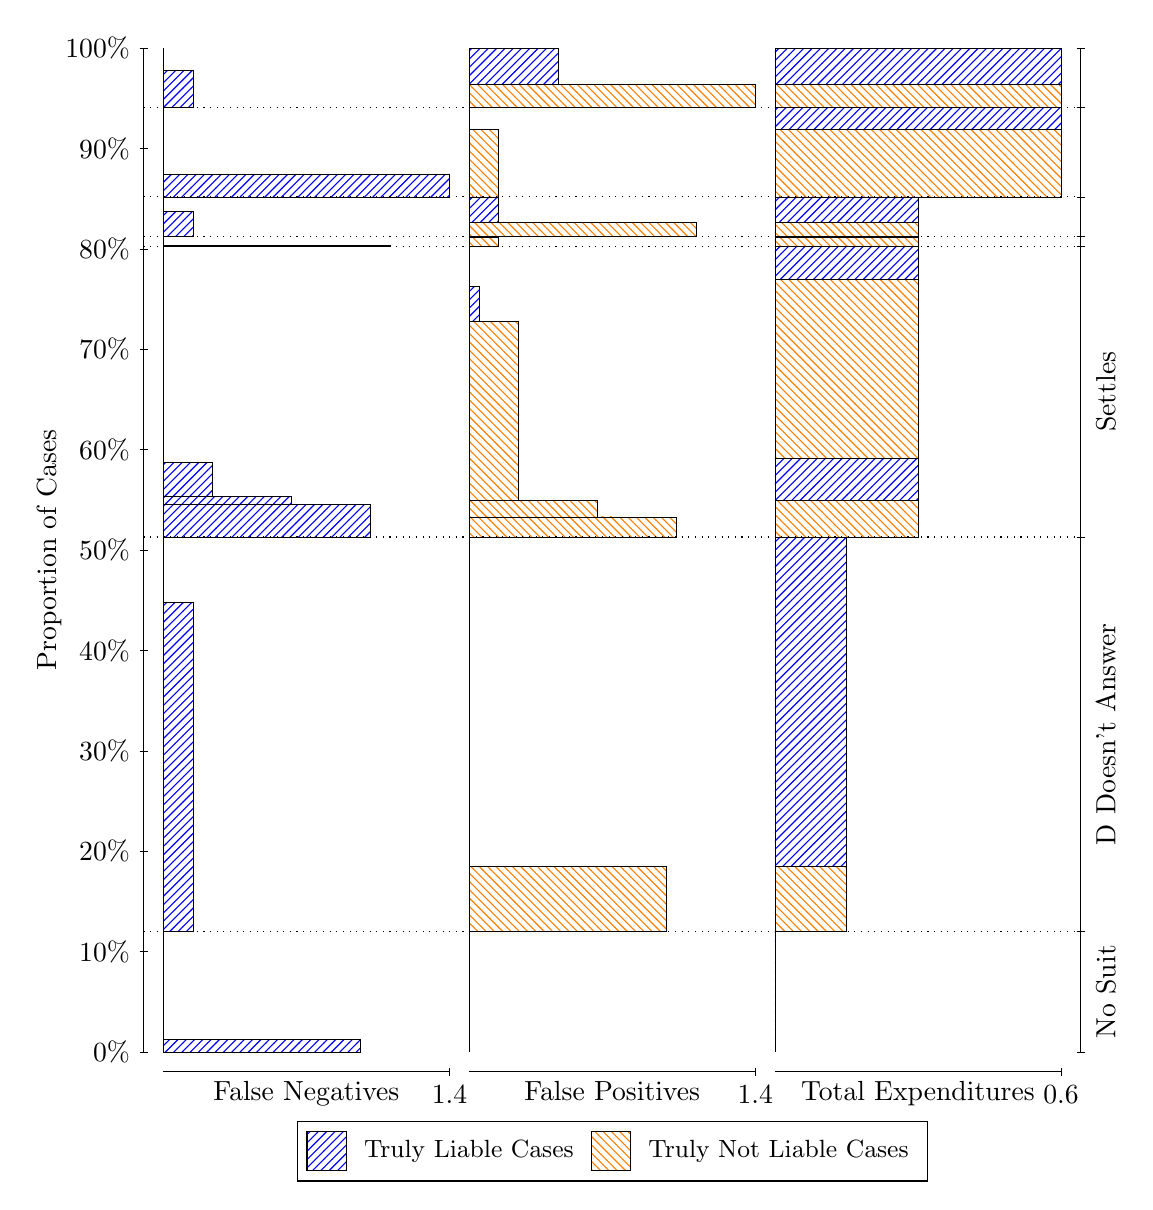
\begin{tikzpicture}
\draw[black, very thin] (1.5,1.75) -- (1.5,14.5);
\node[rotate=90, anchor=center] at (0.3, 8.125) {Proportion of Cases};
\draw[black, very thin] (1.45,1.75) -- (1.55,1.75);
\node[anchor=east] at (1.45, 1.75) {0\%};
\draw[black, very thin] (1.45,3.025) -- (1.55,3.025);
\node[anchor=east] at (1.45, 3.025) {10\%};
\draw[black, very thin] (1.45,4.3) -- (1.55,4.3);
\node[anchor=east] at (1.45, 4.3) {20\%};
\draw[black, very thin] (1.45,5.575) -- (1.55,5.575);
\node[anchor=east] at (1.45, 5.575) {30\%};
\draw[black, very thin] (1.45,6.85) -- (1.55,6.85);
\node[anchor=east] at (1.45, 6.85) {40\%};
\draw[black, very thin] (1.45,8.125) -- (1.55,8.125);
\node[anchor=east] at (1.45, 8.125) {50\%};
\draw[black, very thin] (1.45,9.4) -- (1.55,9.4);
\node[anchor=east] at (1.45, 9.4) {60\%};
\draw[black, very thin] (1.45,10.675) -- (1.55,10.675);
\node[anchor=east] at (1.45, 10.675) {70\%};
\draw[black, very thin] (1.45,11.95) -- (1.55,11.95);
\node[anchor=east] at (1.45, 11.95) {80\%};
\draw[black, very thin] (1.45,13.225) -- (1.55,13.225);
\node[anchor=east] at (1.45, 13.225) {90\%};
\draw[black, very thin] (1.45,14.5) -- (1.55,14.5);
\node[anchor=east] at (1.45, 14.5) {100\%};

\draw[black, very thin] (13.4,1.75) -- (13.4,14.5);
\draw[black, very thin] (13.35,1.75) -- (13.45,1.75);
\node[anchor=west] at (13.35, 1.75) {};
\draw[black, very thin] (13.35,3.2812) -- (13.45,3.2812);
\node[anchor=west] at (13.35, 3.2812) {};
\draw[black, very thin] (13.35,8.2901) -- (13.45,8.2901);
\node[anchor=west] at (13.35, 8.2901) {};
\draw[black, very thin] (13.35,11.981) -- (13.45,11.981);
\node[anchor=west] at (13.35, 11.981) {};
\draw[black, very thin] (13.35,12.105) -- (13.45,12.105);
\node[anchor=west] at (13.35, 12.105) {};
\draw[black, very thin] (13.35,12.609) -- (13.45,12.609);
\node[anchor=west] at (13.35, 12.609) {};
\draw[black, very thin] (13.35,13.75) -- (13.45,13.75);
\node[anchor=west] at (13.35, 13.75) {};
\draw[black, very thin] (13.35,14.5) -- (13.45,14.5);
\node[anchor=west] at (13.35, 14.5) {};

\draw[black, very thin, pattern color=blue, pattern=north east lines] (1.75,1.75) rectangle (4.2557,1.9111);
\draw[black, very thin, pattern color=orange, pattern=north west lines] (1.75,1.9111) rectangle (1.75,3.2812);
\draw[black, very thin, pattern color=blue, pattern=north east lines] (1.75,3.2812) rectangle (2.1259,7.4626);
\draw[black, very thin, pattern color=orange, pattern=north west lines] (1.75,7.4626) rectangle (1.75,8.2901);
\draw[black, very thin, pattern color=blue, pattern=north east lines] (1.75,8.2901) rectangle (4.381,8.7076);
\draw[black, very thin, pattern color=blue, pattern=north east lines] (1.75,8.7076) rectangle (3.3787,8.8014);
\draw[black, very thin, pattern color=blue, pattern=north east lines] (1.75,8.8014) rectangle (3.1282,8.8021);
\draw[black, very thin, pattern color=blue, pattern=north east lines] (1.75,8.8021) rectangle (2.8776,8.8028);
\draw[black, very thin, pattern color=blue, pattern=north east lines] (1.75,8.8028) rectangle (2.627,8.8036);
\draw[black, very thin, pattern color=blue, pattern=north east lines] (1.75,8.8036) rectangle (2.3764,9.2411);
\draw[black, very thin, pattern color=orange, pattern=north west lines] (1.75,9.2411) rectangle (1.75,11.981);
\draw[black, very thin, pattern color=blue, pattern=north east lines] (1.75,11.981) rectangle (4.6316,11.992);
\draw[black, very thin, pattern color=orange, pattern=north west lines] (1.75,11.992) rectangle (1.75,12.105);
\draw[black, very thin, pattern color=blue, pattern=north east lines] (1.75,12.105) rectangle (2.1259,12.425);
\draw[black, very thin, pattern color=orange, pattern=north west lines] (1.75,12.425) rectangle (1.75,12.609);
\draw[black, very thin, pattern color=blue, pattern=north east lines] (1.75,12.609) rectangle (5.3833,12.897);
\draw[black, very thin, pattern color=orange, pattern=north west lines] (1.75,12.897) rectangle (1.75,13.75);
\draw[black, very thin, pattern color=blue, pattern=north east lines] (1.75,13.75) rectangle (2.1259,14.213);
\draw[black, very thin, pattern color=orange, pattern=north west lines] (1.75,14.213) rectangle (1.75,14.5);
\draw[black, very thin, pattern color=orange, pattern=north west lines] (5.6333,1.75) rectangle (5.6333,3.1201);
\draw[black, very thin, pattern color=blue, pattern=north east lines] (5.6333,3.1201) rectangle (5.6333,3.2812);
\draw[black, very thin, pattern color=orange, pattern=north west lines] (5.6333,3.2812) rectangle (8.1391,4.1086);
\draw[black, very thin, pattern color=blue, pattern=north east lines] (5.6333,4.1086) rectangle (5.6333,8.2901);
\draw[black, very thin, pattern color=orange, pattern=north west lines] (5.6333,8.2901) rectangle (8.2644,8.5363);
\draw[black, very thin, pattern color=orange, pattern=north west lines] (5.6333,8.5363) rectangle (8.0138,8.5398);
\draw[black, very thin, pattern color=orange, pattern=north west lines] (5.6333,8.5398) rectangle (7.7632,8.5432);
\draw[black, very thin, pattern color=orange, pattern=north west lines] (5.6333,8.5432) rectangle (7.5126,8.5465);
\draw[black, very thin, pattern color=orange, pattern=north west lines] (5.6333,8.5465) rectangle (7.2621,8.7594);
\draw[black, very thin, pattern color=orange, pattern=north west lines] (5.6333,8.7594) rectangle (6.2598,11.031);
\draw[black, very thin, pattern color=blue, pattern=north east lines] (5.6333,11.031) rectangle (5.7586,11.468);
\draw[black, very thin, pattern color=blue, pattern=north east lines] (5.6333,11.468) rectangle (5.6333,11.981);
\draw[black, very thin, pattern color=orange, pattern=north west lines] (5.6333,11.981) rectangle (6.0092,12.095);
\draw[black, very thin, pattern color=blue, pattern=north east lines] (5.6333,12.095) rectangle (5.6333,12.105);
\draw[black, very thin, pattern color=orange, pattern=north west lines] (5.6333,12.105) rectangle (8.5149,12.289);
\draw[black, very thin, pattern color=blue, pattern=north east lines] (5.6333,12.289) rectangle (6.0092,12.609);
\draw[black, very thin, pattern color=orange, pattern=north west lines] (5.6333,12.609) rectangle (6.0092,13.462);
\draw[black, very thin, pattern color=blue, pattern=north east lines] (5.6333,13.462) rectangle (5.6333,13.75);
\draw[black, very thin, pattern color=orange, pattern=north west lines] (5.6333,13.75) rectangle (9.2667,14.037);
\draw[black, very thin, pattern color=blue, pattern=north east lines] (5.6333,14.037) rectangle (6.7609,14.5);
\draw[black, very thin, pattern color=orange, pattern=north west lines] (9.5167,1.75) rectangle (9.5167,3.1201);
\draw[black, very thin, pattern color=blue, pattern=north east lines] (9.5167,3.1201) rectangle (9.5167,3.2812);
\draw[black, very thin, pattern color=orange, pattern=north west lines] (9.5167,3.2812) rectangle (10.425,4.1086);
\draw[black, very thin, pattern color=blue, pattern=north east lines] (9.5167,4.1086) rectangle (10.425,8.2901);
\draw[black, very thin, pattern color=orange, pattern=north west lines] (9.5167,8.2901) rectangle (11.333,8.7594);
\draw[black, very thin, pattern color=blue, pattern=north east lines] (9.5167,8.7594) rectangle (11.333,9.2929);
\draw[black, very thin, pattern color=orange, pattern=north west lines] (9.5167,9.2929) rectangle (11.333,11.564);
\draw[black, very thin, pattern color=blue, pattern=north east lines] (9.5167,11.564) rectangle (11.333,11.981);
\draw[black, very thin, pattern color=orange, pattern=north west lines] (9.5167,11.981) rectangle (11.333,12.095);
\draw[black, very thin, pattern color=blue, pattern=north east lines] (9.5167,12.095) rectangle (11.333,12.105);
\draw[black, very thin, pattern color=orange, pattern=north west lines] (9.5167,12.105) rectangle (11.333,12.289);
\draw[black, very thin, pattern color=blue, pattern=north east lines] (9.5167,12.289) rectangle (11.333,12.609);
\draw[black, very thin, pattern color=orange, pattern=north west lines] (9.5167,12.609) rectangle (13.15,13.462);
\draw[black, very thin, pattern color=blue, pattern=north east lines] (9.5167,13.462) rectangle (13.15,13.75);
\draw[black, very thin, pattern color=orange, pattern=north west lines] (9.5167,13.75) rectangle (13.15,14.037);
\draw[black, very thin, pattern color=blue, pattern=north east lines] (9.5167,14.037) rectangle (13.15,14.5);
\draw[black, dotted] (1.5,3.2812) -- (13.4,3.2812);
\draw[black, dotted] (1.5,8.2901) -- (13.4,8.2901);
\draw[black, dotted] (1.5,11.981) -- (13.4,11.981);
\draw[black, dotted] (1.5,12.105) -- (13.4,12.105);
\draw[black, dotted] (1.5,12.609) -- (13.4,12.609);
\draw[black, dotted] (1.5,13.75) -- (13.4,13.75);
\draw[black, very thin] (1.75,1.5) -- (5.3833,1.5);
\node[anchor=north] at (3.5667, 1.5) {False Negatives};
\draw[black, very thin] (5.3833,1.45) -- (5.3833,1.55);
\node[anchor=north] at (5.3833, 1.45) {1.4};

\draw[black, very thin] (5.6333,1.5) -- (9.2667,1.5);
\node[anchor=north] at (7.45, 1.5) {False Positives};
\draw[black, very thin] (9.2667,1.45) -- (9.2667,1.55);
\node[anchor=north] at (9.2667, 1.45) {1.4};

\draw[black, very thin] (9.5167,1.5) -- (13.15,1.5);
\node[anchor=north] at (11.333, 1.5) {Total Expenditures};
\draw[black, very thin] (13.15,1.45) -- (13.15,1.55);
\node[anchor=north] at (13.15, 1.45) {0.6};

\node[black, centered, rotate=90] at (13.72, 2.5156) {No Suit};
\node[black, centered, rotate=90] at (13.72, 5.7856) {D Doesn't Answer};
\node[black, centered, rotate=90] at (13.72, 10.136) {Settles};





\draw (7.449999999999999,1.5) node[draw=none] (baseCoordinate) {};
\begin{scope}[align=center]
        \matrix[scale=0.5, draw=black, below=0.5cm of baseCoordinate, nodes={draw}, column sep=0.1cm]{
            \node[rectangle, draw, minimum width=0.5cm, minimum height=0.5cm, pattern=north east lines, pattern color=blue] {}; &
            \node[draw=none, font=\small] (B) {Truly Liable Cases}; &
            \node[rectangle, draw, minimum width=0.5cm, minimum height=0.5cm, pattern=north west lines, pattern color=orange] {}; &
            \node[draw=none, font=\small] (B) {Truly Not Liable Cases}; \\
            };
\end{scope}

\end{tikzpicture}
\end{document}